\documentclass{article}
\usepackage[utf8]{inputenc}
\usepackage[russian]{babel}
\usepackage{graphicx}
\usepackage{indentfirst}
\newcommand{\degree}{^{\circ}}
%Tennis racket theorem
\title{Об эффекте Джанибекова (англ. Tennis racket theorem)}
\date{\today}
\author{А.~Г.~Петров, С.~Е.~Володин}
\begin{document}
\maketitle
\section{Введение}
Космонавт Джанибеков наблюдал неожиданное движение гайки в космосе при определенных условиях. Быстро вращаясь вокруг некоторой оси, гайка совершала <<кувырок>>~--- ось быстрого вращения <<скачком>> поворачивалась на \begin{math} 180\degree \end{math}. Этот эффект также можно получить и на Земле (например, подбрасывая в воздух теннисную ракетку).
\section{Уравнения Эйлера}
Для описания вращательного движения тела удобно использовать уравнения Эйлера. Получим их.
Пусть тело совершает вращение при отсутствии внешних моментов сил.
\begin{math}
\vec{e1}, \vec{e2}, \vec{e3}
\end{math}~--- базис некоторой ИСО,
\begin{math}
\vec{i}, \vec{j}, \vec{k}
\end{math}~--- базис СО, связанной с телом, причем ее оси совпадают с главными осями тела и
\begin{equation}
J=\left( \begin{array}{lcr} A & 0 & 0\\ 0 & B & 0\\ 0 & 0 & C \end{array} \right),\ A > B > C,
\end{equation}
где A, B, C~--- моменты инерции тела в главных осях, а \begin{math} J \end{math}~--- тензор инерции. Если \begin{math} \vec{\omega} \end{math}~--- вектор угловой скорости, то можно обозначить его компоненты в подвижных осях:
\begin{equation}
\vec{\omega}=
\left( \begin{array}{lcr} \vec{i} & \vec{j} & \vec{k} \end{array} \right)
\left( \begin{array}{lcr} p\\q\\r \end{array} \right)
\end{equation}
И если \begin{math} \vec{K} \end{math}~--- вектор момента импульса, то
\begin{equation}
\vec{K}=J\vec{\omega}=
\left( \begin{array}{lcr} \vec{i} & \vec{j} & \vec{k} \end{array} \right)
\left( \begin{array}{lcr} A p\\B q\\C r \end{array} \right)
\end{equation}
Но если \begin{math} \vec{M} \end{math}~--- момент внешних сил, то в ИСО
\begin{equation}
\frac{d\vec{K}}{dt}=\vec{M}=0
\end{equation}
Тогда получаем
\begin{equation}
\frac{d\vec{K}}{dt}=
\frac{d\left( \begin{array}{lcr} \vec{i} & \vec{j} & \vec{k} \end{array} \right)}{dt}\left( \begin{array}{lcr} A p\\B q\\C r \end{array} \right)+
\left( \begin{array}{lcr} \vec{i} & \vec{j} & \vec{k} \end{array} \right)\frac{d\left( \begin{array}{lcr} A p\\B q\\C r \end{array} \right)}{dt}=
[\vec{\omega}, \vec{K}] + \left( \begin{array}{lcr} \vec{i} & \vec{j} & \vec{k} \end{array} \right)\frac{d\left( \begin{array}{lcr} A p\\B q\\C r \end{array} \right)}{dt},
\end{equation}
что в проекциях на подвижные оси может быть записано как
% ( i   j   k )
% ( p  q   r )
% (ApBqCr)
% 
% rq(C - B)
% pr(A - C)
% qp(B - A)
\begin{equation}
\label{EulerEquations}
\left\{
\begin{array}{c}
A\frac{dp}{dt}+rq(C-B)=0\\
B\frac{dq}{dt}+pr(A-C)=0\\
C\frac{dr}{dt}+qp(B-A)=0
\end{array}
\right.
.
\end{equation}
Эти уравнения и называются уравнениями Эйлера.
\section{Расчет моментов инерции гайки}
%решение с эллипсом (численное)
%решение с материальными точками, отстоящими на радиус инерции
\section{Геометрическая интерпретация Мак-Кулага}
%\begin{figure}
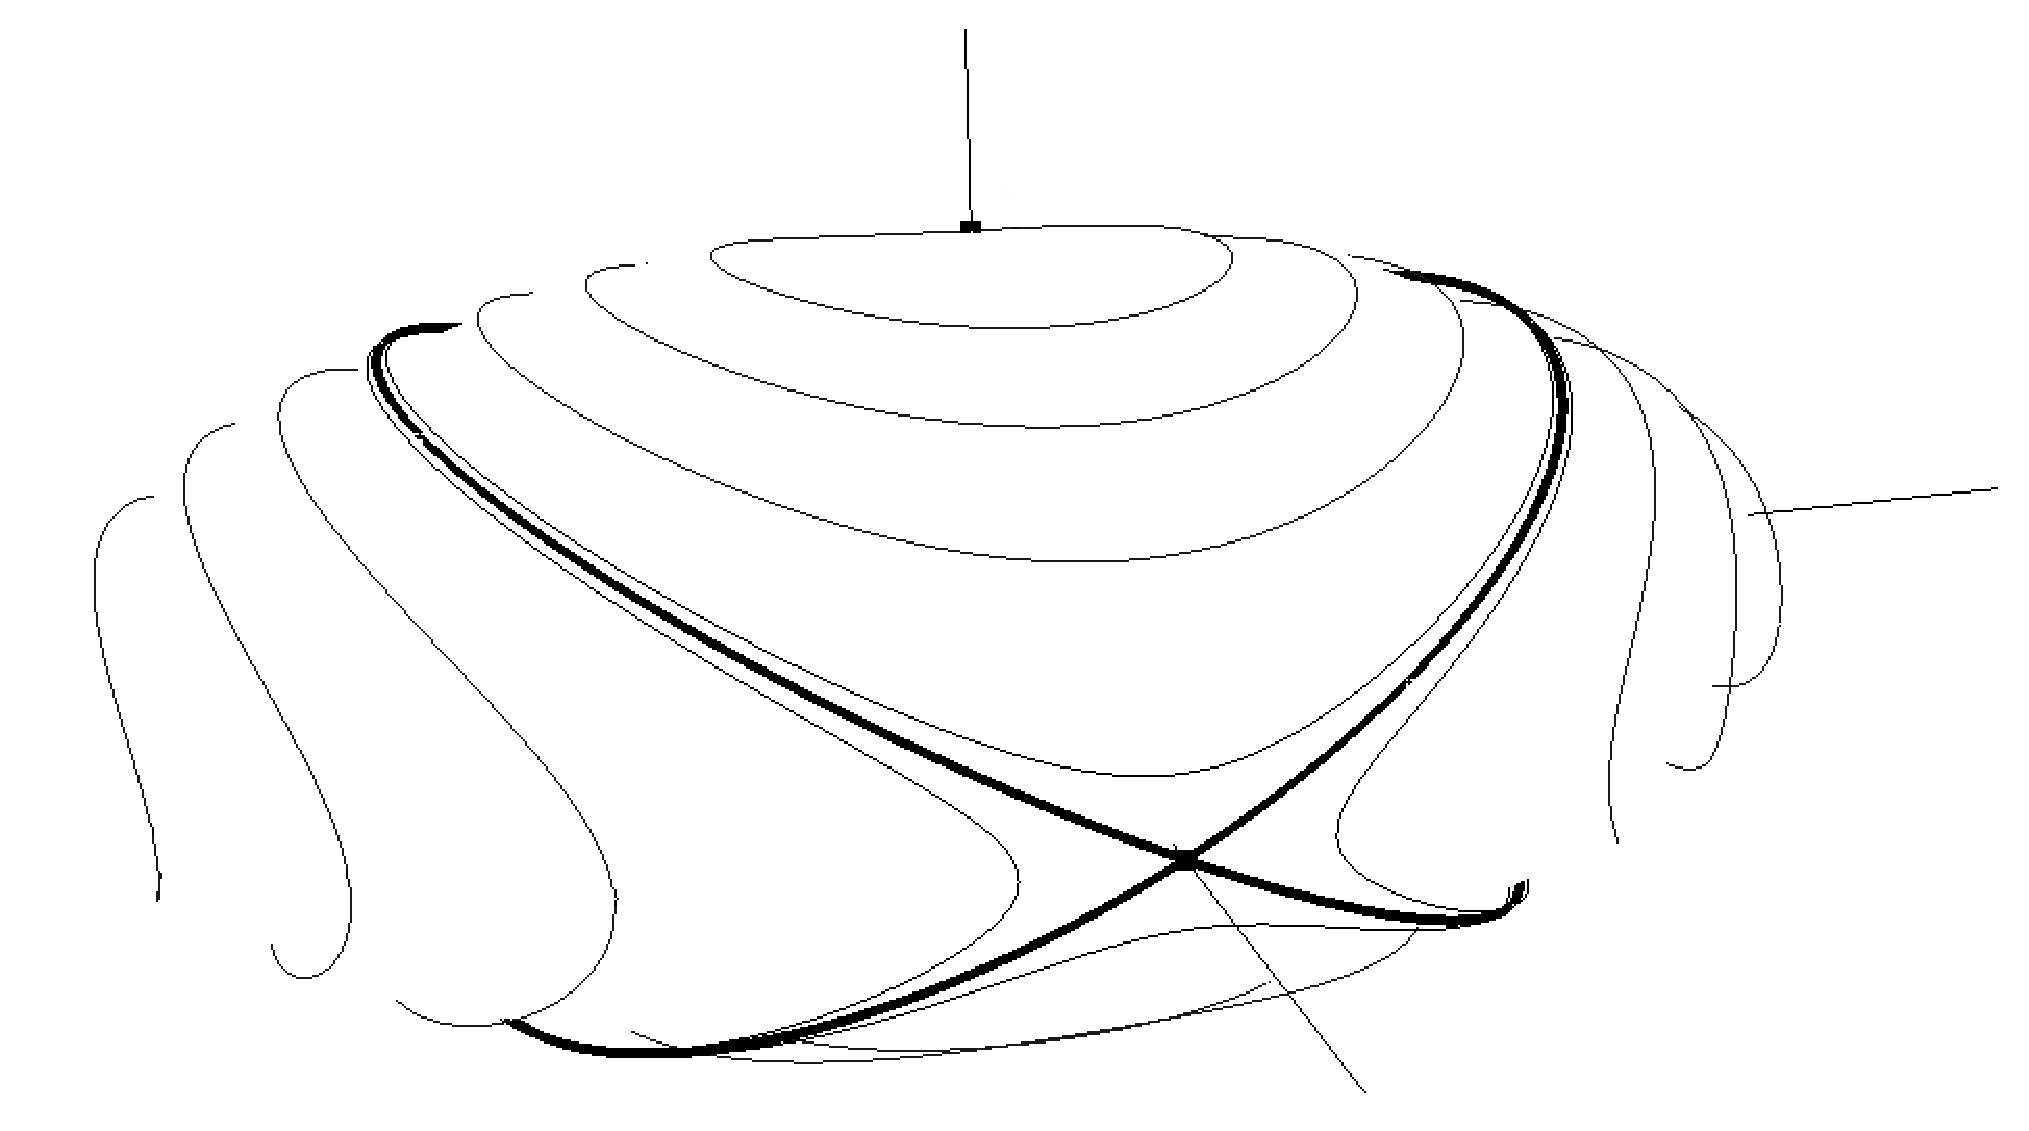
\includegraphics[height=5cm]{ellipsoid}
\newline
%\caption{Подпись к рисунку} \label{fig:2}
%\end{figure}
%нужно написать _перед_ уравнениями Эйлера, потому что иначе непонятно, почему интересна именно средняя компонента q угловой скорости
%пересечение эллипсоида и сфера в пространстве моментов импульса.
%добавить картинку
Получим наглядное представление вращательного движения. Для начала запишем закон сохранения момента импульса \begin{math} \vec{K} \end{math} и энергии \begin{math} T \end{math}:
\begin{equation}
\label{angularMomentumInv}
\vec{K}^2\equiv A^2p^2+B^2q^2+C^2r^2=const
\end{equation}
\begin{equation}
\label{energyInv}
2T\equiv\frac{1}{2}\left(\vec{K},\vec{\omega}\right)=A^2p+B^2q+C^2r=const
\end{equation}
Обозначив компоненты вектора \begin{math} \vec{K} \end{math} за
\begin{equation}
\vec{K}=
\left(
\begin{array}{lcr}
\vec{i} & \vec{j} & \vec{k}
\end{array}
\right)
\left(
\begin{array}{lcr}
X\\
Y\\
Z
\end{array}
\right),
X=Ap,Y=Bq,Z=Cr,
\end{equation}
\begin{equation}
\left\{
\begin{array}{l}
\ref{angularMomentumInv}\\
\ref{energyInv}
\end{array}
\right.
\Leftrightarrow
\left\{
\begin{array}{l}
X^2+Y^2+Z^2=K^2\\
X^2/A+Y^2/B+Z^2/C=2T
\end{array}
\right.
\end{equation}
Эти уравнения являются уравнениями сфера радиуса \begin{math} \vec{K}^2 \end{math} и эллипсоида с полуосями \begin{math} \sqrt{2TA}, \sqrt{2TB}, \sqrt{2TC} \end{math}, а система является их пересечением. Поскольку вектор \begin{math} \vec{K} \end{math} неподвижен в пространстве, а тело совершает вращение, кривая пересечения совпадает с кривой, которую описывает в пространстве некоторая точка тела (в ИСО).
\section{Интегралы уравнений Эйлера}
%получить выражения для q как интеграл по времени
Поставим задачу получить уравнение для \begin{math} t, q \end{math}. 
Выражение для компоненты угловой скорости \begin{math} q \end{math} можно получить, решив систему
\begin{math}
\left\{
\begin{array}{l}
\ref{angularMomentumInv}\\
\ref{energyInv}
\end{array}
\right.
\end{math}
относительно \begin{math} p^2, r^2\end{math} и обозначив соответствующие постоянные во времени коэффициенты за \begin{math} a, b, c, d \end{math}:
% ( A   C   )(p^2) = (2T-Bq^2   )
% ( A^2 C^2 )(r^2)   (K^2-B^2q^2)
\begin{equation}
\begin{array}{l}
\Delta=AC(C-A)<0\\
p^2=\frac{C^2(2T-Bq^2)-C(K^2-B^2q^2)}{\Delta}=a-bq^2\\
q^2=\frac{A(K^2-B^2q^2)-A^2(2T-Bq^2)}{\Delta}=c-dq^2
\end{array}.
\end{equation}
Тогда, подставив эти выражения во второе уравнение Эйлера \ref{EulerEquations}:
\begin{equation}
B\frac{dq}{dt}\pm(A-C)\sqrt{(a-bq^2)(c-dq^2)}=0,
\end{equation}
можно получить выражение для времени:
\begin{equation}
\Delta t=\pm\frac{B}{A-C}{\int\limits_{q1}^{q2}\frac{dq}{\sqrt{(a-bq^2)(c-dq^2)}}}.
\end{equation}
Это уравнение позволяет получить время между теми состояниями, при которых вторая компонента угловой скорости \begin{math} q \end{math} равна \begin{math} q2 \end{math} и \begin{math} q1 \end{math} соответственно.
%Знак \begin{math} \pm \end{math} проще всего определить, когда величины \begin{math} p, r \end{math} сами не меняют знака.
\section{Решение задачи при движении по сепаратрисе}
%бесконечное время, не очень полезные формулы
\section{Решение задачи при движении вблизи сепаратрисы}
%K^2-2TB=eps
\subsection{Период движения}
%приведение к виду, который решает Wolfram Mathematica
%асимптотическое решение при eps->0
\subsection{Время переворота}
%тот же интеграл, что и в периоде, но другие пределы интегрирования.
\end{document}